% F1 — Host-level architecture
% Standalone TikZ figure: compile with lualatex or pdflatex.
% The enclosing chapter supplies \caption{}; no caption text lives here.
\documentclass[tikz,border=5pt]{standalone}
\usetikzlibrary{positioning, arrows.meta, shapes.geometric, backgrounds, fit, calc}

\begin{document}
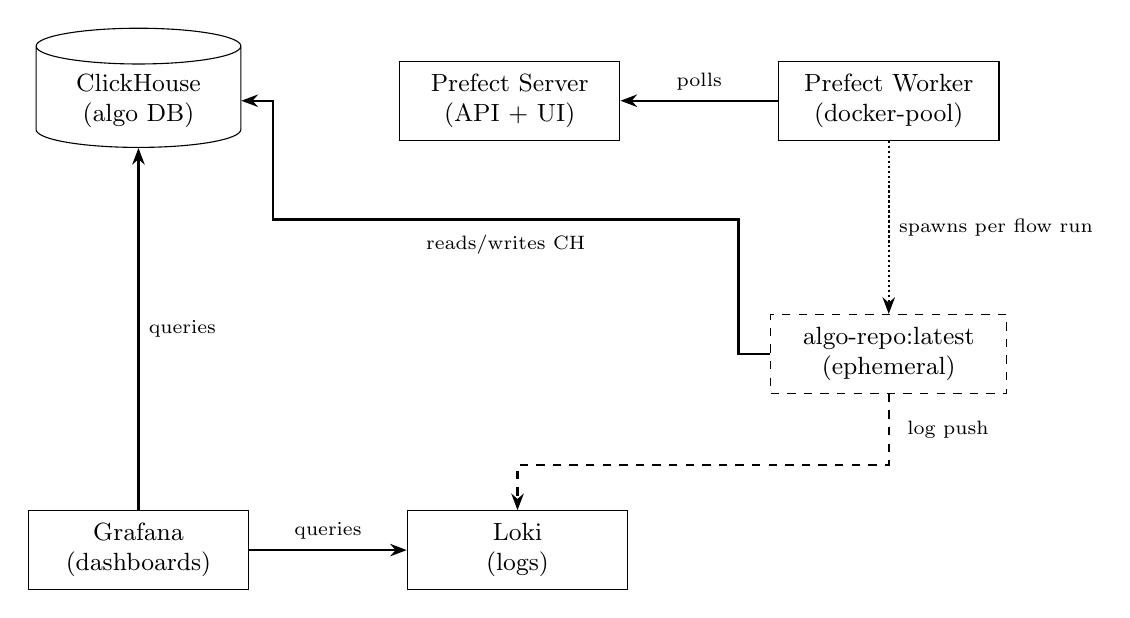
\begin{tikzpicture}[
  % --- node styles ---
  service/.style={
    draw, rectangle,
    minimum width=2.8cm, minimum height=1.0cm,
    align=center, font=\small
  },
  db/.style={
    draw, cylinder,
    shape border rotate=90,
    minimum width=2.6cm, minimum height=1.0cm,
    align=center, font=\small,
    aspect=0.25
  },
  ephemeral/.style={
    draw, rectangle, dashed,
    minimum width=3.0cm, minimum height=1.0cm,
    align=center, font=\small
  },
  hostbox/.style={
    draw, rectangle,
    inner sep=20pt
  },
  % --- arrow styles ---
  solid/.style={-{Stealth[length=6pt]}, thick},
  dashed_arr/.style={-{Stealth[length=6pt]}, thick, dashed},
  spawns/.style={-{Stealth[length=6pt]}, thick, densely dotted}
]

% ---- long-lived services (top row) ----
\node[db]      (ch)      {ClickHouse\\(algo DB)};
\node[service] (server)  [right=2.0cm of ch]    {Prefect Server\\(API + UI)};
\node[service] (worker)  [right=2.0cm of server]{Prefect Worker\\(docker-pool)};

% ---- ephemeral container (below worker) ----
\node[ephemeral] (algo)  [below=2.2cm of worker]
    {algo-repo:latest\\(ephemeral)};

% ---- observability row (well below upper services) ----
\node[service] (grafana) [below=4.6cm of ch]    {Grafana\\(dashboards)};
\node[service] (loki)    [right=2.0cm of grafana]{Loki\\(logs)};

% ---- arrows ----

% Prefect Worker polls Prefect Server (solid)
\draw[solid] (worker.west) -- (server.east)
    node[midway, above, font=\scriptsize] {polls};

% Prefect Worker spawns ephemeral container (dotted, labelled)
\draw[spawns] (worker.south) -- (algo.north)
    node[midway, right, font=\scriptsize] {spawns per flow run};

% Ephemeral container reads/writes ClickHouse (solid).
% Exits algo on its west side, routes UP a short distance, LEFT under the
% Prefect Server box, then UP again on the left and into ch.east — so the
% horizontal passes BENEATH Prefect Server with no overlap.
\coordinate (alg_w)         at ([xshift=-0.4cm]algo.west);
\coordinate (under_top_row) at ([yshift=-1.0cm]server.south);
\coordinate (under_right)   at (alg_w           |- under_top_row);
\coordinate (under_left)    at ([xshift=0.4cm]ch.east |- under_top_row);
\coordinate (e_off)         at ([xshift=0.4cm]ch.east);
\draw[solid] (algo.west) -- (alg_w) -- (under_right) -- (under_left) -- (e_off) -- (ch.east);
\node[font=\scriptsize, below=2pt] at ($(under_right)!0.5!(under_left)$) {reads/writes CH};

% Ephemeral container pushes logs to Loki (dashed).
% Label sits on the vertical leg, well clear of the long horizontal
% dashed segment that ends at loki.north.
\draw[dashed_arr] (algo.south)
    -- node[right=3pt, font=\scriptsize] {log push} ++(0,-0.9)
    -| (loki.north);

% Grafana queries Loki (solid)
\draw[solid] (grafana.east) -- (loki.west)
    node[midway, above, font=\scriptsize] {queries};

% Grafana queries ClickHouse (solid) — enters ClickHouse from below
% (south), so the two arrows hitting ClickHouse use clearly different
% sides (algo enters from east, grafana enters from south).
\draw[solid] (grafana.north) -- (ch.south)
    node[midway, right, font=\scriptsize] {queries};

\end{tikzpicture}
\end{document}
